\chapter{Event and Alarm API Example}

The Event and Alarm API Example is a simple demo that shows the usage of the
following primitives:
\begin{itemize}
\item \fn{WaitEvent};
\item \fn{GetEvent};
\item \fn{ClearEvent};
\item \fn{SetEvent};
\item \fn{ErrorHook};
\item \fn{StartupHook};
\item \fn{SetRelAlarm};
\item \fn{CounterTick}.
\end{itemize}

\section{Demo structure}

The demo consists of two tasks, \fn{Task1} and \fn{Task2}.

\fn{Task1} is an \emph{extended task}. Extended tasks are tasks that:
\begin{itemize}
\item can call blocking primitives (in our case, wait for events using
  the \fn{WaitEvent} primitive;
\item {\em must} have a separate stack (because they may suspend upon
a call to a blocking primitive).
\end{itemize}
A task is considered an Extended Task when the OIL file includes
events inside the task properties. In this example, \fn{Task1} is an
extended task because its properties contain the following lines:

\begin{lstlisting}
TASK Task1 {
  ...
  EVENT = "TimerEvent";
  EVENT = "ButtonEvent";
};
\end{lstlisting}

\fn{Task1} waits for two events:
\begin{itemize}
\item A \const{TimerEvent}. The action related to this event is the
  blinking of LED 1. The event is set by a periodic alarm notification
  \const{AlarmTask1} defined in the OIL file.

\item A \const{ButtonEvent}. The action related to this event is the
  blinking of LED 2. The button event is set explicitly using the
  \fn{SetEvent} primitive inside the button interrupt handler.
\end{itemize}

The buttons available on the evaluation board are attached to an
interrupt handler. This interrupt handler sets a relative one-shot
alarm \const{AlarmTask2}. The alarm notification of \const{AlarmTask2}
activates \fn{Task2}. \fn{Task2} simply turns LED 3 on.

The demo also includes an \fn{ErrorHook}. To understand the usage of
\fn{ErrorHook}, please place a breakpoint in the \fn{ErrorHook}
function. Every time an error appears in the execution of a \ee\
primitive, then \fn{ErrorHook} will be called. In the demo, such a
condition appears when the button is pressed rapidly twice. In that
case, a few button interrupts will be generated, and each execution of
the interrupt handler will call the \fn{SetRelAlarm} primitive. When
\fn{SetRelAlarm} will try to activate an alarm already armed, then
\fn{ErrorHook} will be called with a parameter \const{E_OS_STATE}.

The alarm support in \ee\ is basically a wakeup mechanism that can be
attached to application or external events (such as timer interrupts)
to implement an asynchronous notification. In this example, the \ee\
alarm support is used to implement a replacement of the Altera HAL
alarm feature. To obtain this feature, the demo programs the
\const{HIGH_RES_TIMER} timer to periodically raise an interrupt.
\begin{warning}
To run this demo, the Altera System Library project should specify
\const{none} as Timestamp timer.  In this way, we are sure that the
High Res Timer will not be registered by the Altera HAL.
\end{warning}
The timer interrupt calls the \fn{CounterTick} function. The
\fn{CounterTick} function simply increments the counter passed as
parameter, checking if any pending Alarm notification has to be
executed.

Please note that \fn{CounterTick} can be attached to any
source of interrupt, and can be called from any point of your
application to implement user-defined wakeup mechanisms.

The demo contains a \fn{StartupHook}, which contains the
registration of the timer and button interrupts.

Finally, please note that \fn{Task1} uses a blocking primitive like
\fn{WaitEvent}. This implies that \fn{Task1} needs a separate stack
for its execution. Therefore, \fn{Task1} properties in the OIL file
include the following lines:
\begin{lstlisting}
TASK Task1 {
  ...
  STACK = PRIVATE_NIOSII {
    SYS_SIZE = 1024;
  };
};
\end{lstlisting}
that basically reserve 1024 bytes for the private stack of \fn{Task1}.

Another interesting feature of \ee\ is the possibility of
reserving a separate stack for the execution of the interrupt
handlers. This feature has been used in the OIL file of this demo,
reserving 512 bytes for the IRQ stack with the with the following
lines:
\begin{lstlisting}
CPU test_application {
  OS EE {
    ...
    CPU_DATA = NIOSII {
      ...
      MULTI_STACK = TRUE {
	IRQ_STACK = TRUE {
	  SYS_SIZE=512;
	};
	DUMMY_STACK = SHARED;
      };
    };
  };
};
\end{lstlisting}

Having an IRQ stack separated from the rest of the stacks allows a
better sizing of task stacks (that does not have to leave space for
IRQ handlers on each separate stack).

\section{Running the example}
Compile and run the application as usual.

\begin{warning}
Please remember the Altera System Library project should specify
\const{none} as Timestamp timer!!!
\end{warning}

The only action done by \fn{main} is to call \fn{StartOS()}, which
registers the two sources of IRQ (the button and the timer),
automatically activates \fn{Task1}, and arms a periodic alarm
\const{AlarmTask1}.

Every time the timer interrupt fires, the counter \const{Counter1}
will be incremented. Every alarm expiration, Alarm \const{AlarmTask1}
will fire, setting the event \const{TimerEvent} on Task \fn{Task1}:
\fn{Task1} wakes up, get the event, and blinks LED 1. The visible
result is that LED 1 periodically blinks on the board.

Now press the button on the board once. An interrupt is generated that activates an interrupt handler that performs  two actions:
\begin{itemize}
\item It arms the alarm \const{AlarmTask2}, whose notification will
  activate \fn{Task2}. Then \fn{Task2} switches LED 3 on and off.
\item It sets an event \const{ButtonEvent} on \fn{Task1}. As a result,
  \fn{Task1} wakes up switching LED 2 on and off.
\end{itemize}

The visible result is that upon a press of the button, LED 2
immediately blinks (meaning \fn{Task1} has been woken up by the
event), and after a while (around 1 second) LED 3 blinks again
(meaning the alarm \const{AlarmTask2} fired activating \fn{Task2}).

If the button is pressed rapidly, an error in \fn{SetRelAlarm} is
raised, executing \fn{ErrorHook}. The visible result in this case is
that {\em all} the LEDs blink signaling the execution of
\fn{ErrorHook}.






\section{Lauterbach Trace32 support}

This demo also shows the integration of \ee\ with the Lauterbach
Trace32 Debugger and Tracer \cite{Lauterbach}.

The integration supported by \ee\ includes the following features:
\begin{itemize}
\item Automatic generation of the Trace32 PRACTICE Debug scripts to
  program the FPGA, and to load the ELF files produced in the IDE.
\item Automatic generation of multicore debug scripts for
  Multicore designs.
\item Kernel awareness support using ORTI files automatically
  generated by \rtd. 
\end{itemize}

To enable all these features, you need to specify a JAM file
name\footnote{JAM is one of the file formats containing the FPGA
  configuration that is accepted by Lauterbach Trace32} inside the OS
section of the OIL file, as well as the specification of the ORTI
sections that should be generated, as follows:

\begin{lstlisting}
CPU test_application {
  OS EE {
    ...
    NIOS2_JAM_FILE = "JAM_filename.jam";
    ORTI_SECTIONS = ALL;
  }
  ...
}
\end{lstlisting}
(\const{ALL} means the generation of all the ORTI information).

As a result of the compilation process, a set of files are produced
inside the \file{Debug} directory (see Table \ref{tab:t32files} for a
detailed list).

%
\begin{table}
\begin{center}
\begin{tabular}{|c|p{8cm}|}
\hline 
File name&
Description\tabularnewline
\hline
\hline 
\file{debug.bat}&
This batch script loads the FPGA hardware and starts a T32 instance
for each CPU. You can double click it on the Nios II IDE to directly
launch the debug session.\tabularnewline
\hline 
\file{debug\_nojam.bat}&
This batch script starts a T32 instance for each CPU. You can double
click it on the Nios II IDE to directly launch the debug session.
You can use it if the FPGA has been already programmed with the hardware
contents.\tabularnewline
\hline 
\file{t32.cmm}&
Main PRACTICE script, responsible for loading the JAM file and starting
all the T32 instances on every CPU.\tabularnewline
\hline 
\file{testcase\_data.cmm}&
Internal file used for automatic testcase generation.\tabularnewline
\hline 
\file{t32/{*}}&
Internal PRACTICE scripts. They are a copy of the files inside \file{components/evidence\_ee/ee/pkg/cpu/nios2} \file{/debug/lauterbach/t32}.\tabularnewline
\hline 
\file{cpuname/config.t32}&
Configuration file for T32. Contains the Multicore configuration information.\tabularnewline
\hline 
\file{cpuname/orti.men}&
Trace32 menu automatically generated using the Lauterbach ORTI menu
generator.\tabularnewline
\hline
\file{cpuname/system.orti}&
The ORTI file, for each cpu.\tabularnewline
\hline
\file{cpuname/t32.cmm}&
The main script file executed by each CPU.\tabularnewline
\hline
\end{tabular}
\end{center}

\caption{\label{tab:t32files} Files generated for the Lauterbach Trace32 support ({\em cpuname} is the name of the CPU as specified in the OIL file).}
\end{table}




To run the Trace32 debugger, just double click on the
\file{Debug/debug.bat} file generated during the compilation. The
debugger opens up showing a window similar to the one in Figure
\ref{fig:trace32_splash}. 

%
\begin{figure}
\begin{center}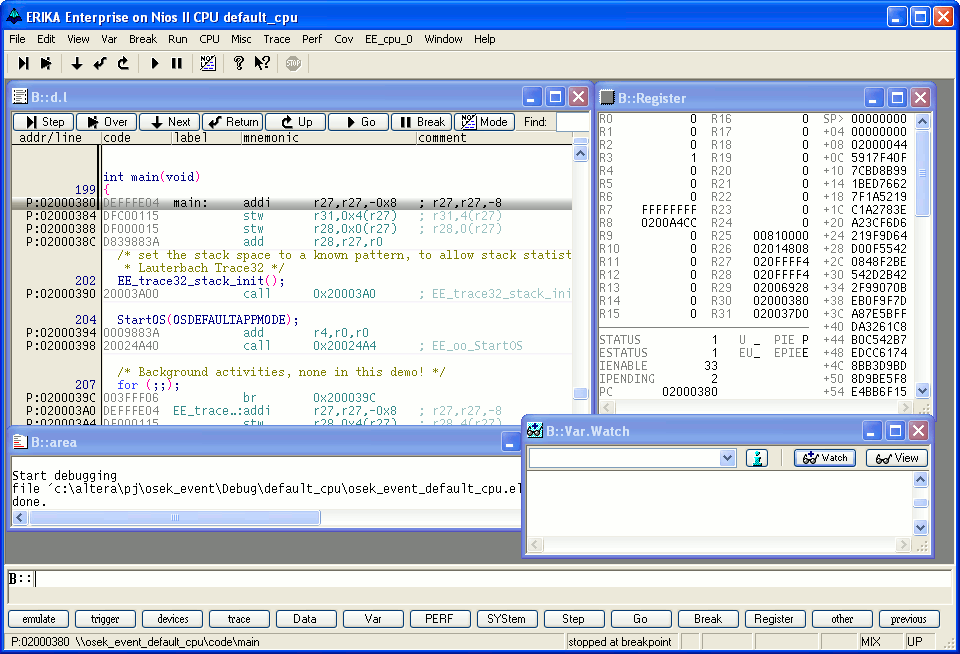
\includegraphics[%
  width=12cm, bb=0 0 960 654]{images/trace32_splash.png}\end{center}
\caption{\label{fig:trace32_splash} The Lauterbach Trace32 for Altera Nios II.}
\end{figure}
%

Please note that each window has a title
with the name of the CPU being under debug. The menu list include a
submenu named ``ee\_cpu\_0'' containing the specification of the ORTI
related debug features.

By clicking on each menu item, you can get useful debug informations
about \ee. In particular:
\begin{itemize}
\item Figure \ref{fig:trace32_os} shows the general information about
  the kernel global variables, such as the name of the running task,
  the current priority of the running task, the last RTOS primitive
  called, the last error returned by an \ee\ primitive, the current
  application mode and the current system ceiling.
%
\begin{figure}
\begin{center}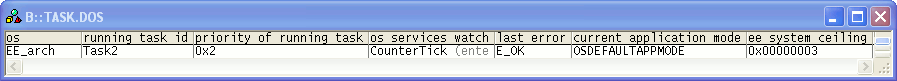
\includegraphics[%
  width=12cm, bb=0 0 897 81]{images/trace32_os.png}\end{center}
\caption{\label{fig:trace32_os} General information about the \ee\ status.}
\end{figure}
%

\item Figure \ref{fig:trace32_task} shows, for each task, the task
  name, its current priority (it may be different from the nominal
  priority when the task lock a resource), the task state, the task
  stack, and the current pending activations.
%
\begin{figure}
\begin{center}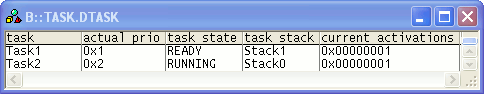
\includegraphics[%
  width=11cm, bb=0 0 484 94]{images/trace32_task.png}\end{center}
\caption{\label{fig:trace32_task} Information about the tasks in the
system.}
\end{figure}
%

\item Figure \ref{fig:trace32_resource} shows, for each resource, the
  resource name, the resource status, the task that has locked the
  resource (if any), and the ceiling priority of the resource.
%
\begin{figure}
\begin{center}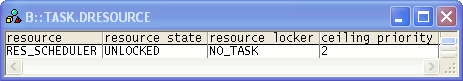
\includegraphics[%
  width=9cm, bb=0 0 463 81]{images/trace32_resource.png}\end{center}
\caption{\label{fig:trace32_resource} Information about the resources
in the system.}
\end{figure}
%

\item Figure \ref{fig:trace32_alarm} shows, for each alarm in the
  system, the alarm name, the time to which the alarm will fire, the
  cycle time of the alarm (\const{0x0} means the alarm is not cyclic),
  the alarm state, the action linked to the alarm notification, the
  counter to which the alarm is attached, and its value.
%
\begin{figure}
\begin{center}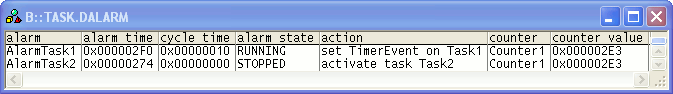
\includegraphics[%
  width=11cm, bb=0 0 673 94]{images/trace32_alarm.png}\end{center}
\caption{\label{fig:trace32_alarm} Information about the alarms in the system.}
\end{figure}
%

\item Finally, Figure \ref{fig:trace32_stack} and Figure
  \ref{fig:trace32_stackview} show information about the stacks that
  has been configured in the application. In particular, the first
  figure shows the stack name, size, base address, direction, and fill
  pattern, while the second figure shows in a graphical way the
  current stack usage. Please remind that to obtain the graphical
  stack usage estimation the application has to call
  \fn{EE_trace32_stack_init} at system startup. In this example,
  \const{Stack0} is the shared stack used by the background task (that
  is, the \fn{main} function), and by \fn{Task2}. \fn{Stack1} is used
  by \fn{Task1}, and \fn{Stack2} is the interrupt stack.
%
\begin{figure}
\begin{center}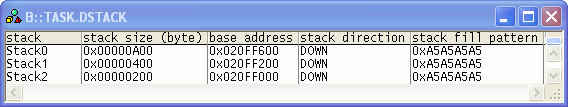
\includegraphics[%
  width=11cm, bb=0 0 568 107]{images/trace32_stack.png}\end{center}
\caption{\label{fig:trace32_stack} The application stack list.}
\end{figure}
%
\begin{figure}
\begin{center}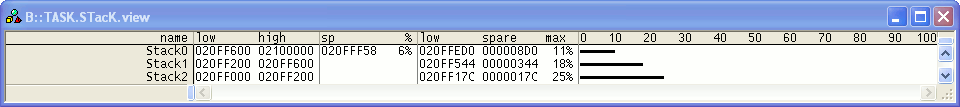
\includegraphics[%
  width=13cm, bb=0 0 960 107]{images/trace32_stackview.png}\end{center}
\caption{\label{fig:trace32_stackview} A graphical view of the
application stack usage.}
\end{figure}

\end{itemize}


The \ee\ Trace32 support also includes support for the Nios II tracer
module. As an example, Figure \ref{fig:trace32_chart_irq} shows the
execution of an interrupt handler as recorded by the tracer
module. Figure \ref{fig:trace32_chart_state} shows an interpretation
of the context changes and task status values using the ORTI
information.

%
\begin{figure}
\begin{center}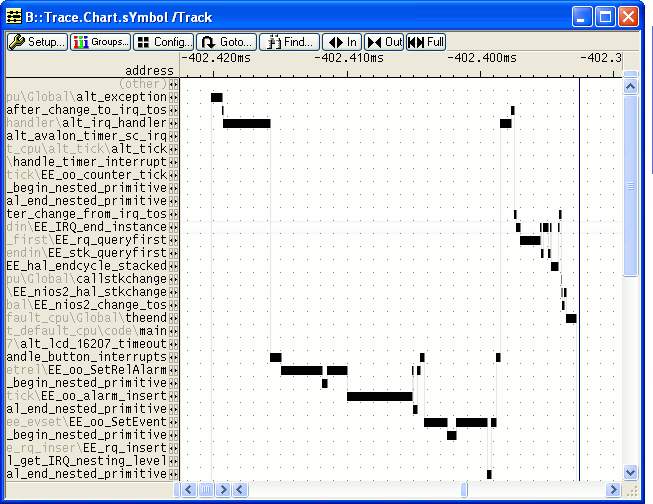
\includegraphics[%
  width=11cm, bb=0 0 653 504]{images/trace32_chart_irq.png}\end{center}
\caption{\label{fig:trace32_chart_irq} The execution of the Button IRQ as recorded by Lauterbach Trace32.}
\end{figure}

%
\begin{figure}
\begin{center}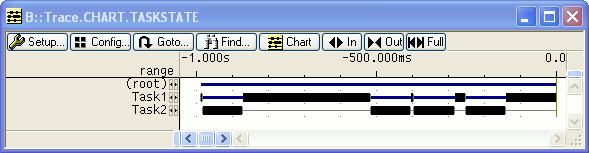
\includegraphics[%
  width=11cm, bb=0 0 589 153]{images/trace32_chart_state.png}\end{center}
\caption{\label{fig:trace32_chart_state} The interpretation of a trace recorded with Lauterbach Trace32 showing the context changes happened in the system.}
\end{figure}

\subsection{Acknowledgements}

We would like to thank Ing. Maurizio Menegotto from Lauterbach Italy
Srl for his support in the integration of \rtd\ and \ee\ with the
Lauterbach Trace32 Debugger and Tracer.

